\section{Changeable parameters on an electric guitar}

In order to give an electric guitar a certain sound, some changes can be made directly by changing physical parts on the guitar. This section aims to give an overview of some of these changeable parameters. These parameters mentioned, are parameters which changes the sound of the guitar, when it is not amplified. The following parameters will be investigated:

\begin{itemize}
 \item String thickness and material
 \item playing with fingers or picks
 \item String action
 \item Bridges
\end{itemize}

To get an overview of how the different parameters influence the sound, a description of an electric guitar will be made.

\subsection{The electric guitar}

In \autoref{fig:guitar_parts} an illustration of an electrical guitar and its parts is shown.

\begin{figure}[h]
	\centering
		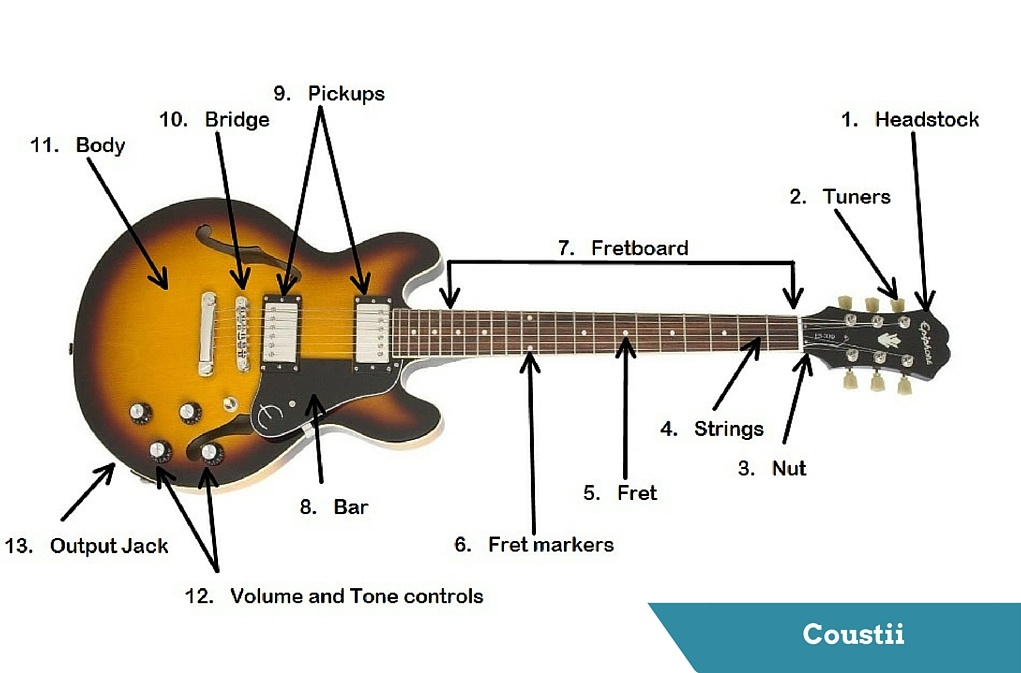
\includegraphics[width=0.9\textwidth]{guitar_parts.jpg}
		\caption{Illustration of an electric guitar and its parts \citep{}.}
		\label{fig:guitar_parts}
\end{figure}
\todo[inline]{Sebastian: Maybe remove blue box?}

In the figure several parts are highlighted, but not all of them influence the sound, in the case where the guitar is not amplified. The pickups, the volume- and the tone-control have a large influence on the sound, when amplified, but they have no influence when not amplified. The Tuners do have an have an influence on the sound, but more in the sense of


